\documentclass[letterpaper,12pt,fleqn]{article}
\usepackage{matharticle}
\usepackage{tikz}
\usepackage{array}
\pagestyle{empty}
\newcommand{\T}{\mathscr{T}}
\newcommand{\U}{\mathcal{U}}
\newcommand{\e}{\epsilon}
\renewcommand{\a}{\alpha}
\renewcommand{\l}{\lambda}
\renewcommand{\C}{\mathcal{C}}
\begin{document}
\section*{Closed Sets}

\begin{notation}
  Let \((X,\T)\) be a topological space and \(p\in X\):
  \[\U_p=\setb{U\in\T}{p\in U}\]
\end{notation}

\begin{definition}[Limit Point]
  Let \((X,\T)\) be a topological space, \(A\subset X\), and \(p\in X\).  To say that \(p\) is a \emph{limit point}
  of \(A\) means:
  \[\forall\,U\in\U_p,(U-\set{p})\cap A\ne\emptyset\]
\end{definition}

\begin{example}
  Let \(X=\R\) and \(A=(1,2)\).  Verify that \(0\) is a limit point of \(A\) in the indiscrete and cofinite
  topologies but not in the standard nor discrete topologies.

  \begin{description}
  \item[Indiscrete:] Since \(0\notin(1,2)\), it follows that \((\R-\set{0})\cap (1,2)=(1,2)\ne\emptyset\).

    Therefore \(0\) is a limit point of \((1,2)\).

  \item[Cofinite:] Assume \(U\in\T\).

    This means that \(U=\R-X\) where \(X\) is some finite set.  But \((1,2)\) is uncountable and so:
    \begin{align*}
      (U-\set{0})\cap(1,2) &= U\cap(1,2) \\
      &= (\R-X)\cap(1,2) \\
      &= (\R\cap(1,2))-(X\cap(1,2)) \\
      &= (1,2)-(X\cap(1,2)) \\
      &\ne\emptyset
    \end{align*}

    Therefore \(0\) is a limit point of \((1,2)\).

  \item[Standard:] Let \(\e=\frac{1}{2}\).

    \(B(0,\frac{1}{2})\cap(1,2)=\emptyset\)

    Therefore \(0\) is not a limit point of \((1,2)\).

  \item[Discrete:] Consider \([0,1]\in\T\).

    \(0\in[0,1]\) but \([0,1]\cap(1,2)=\emptyset\).

    Therefore \(0\) is not a limit point of \((1,2)\).
  \end{description}
\end{example}

\begin{theorem}
  Let \((X,\T)\) be a topological space, \(A\subset X\), and \(p\in X\) but \(p\notin A\).  \(p\) is not a limit
  point of \(A\) iff there exists \(U\in\U_p\) such that \(U\cap A=\emptyset\).
\end{theorem}

\begin{proof}
  If \(p\notin A\) then the definition of a limit point becomes: \(p\) is a limit point of \(A\) iff for all
  \(U\in\U_p,U\cap A\ne\emptyset\).  Negating both sides of the equivalence yields an equivalent proposition and
  gives the desired result.
\end{proof}

\begin{definition}[Isolated Point]
  Let \((X,\T)\) be a topological space, \(A\subset X\), and \(p\in X\).  To say that \(p\) is an \emph{isolated
    point} in \(A\) means that \(p\in A\) and \(p\) is not a limit point of \(A\).
\end{definition}

\begin{theorem}
  Let \((X,\T)\) be a topological space, \(A\subset X\), and \(p\in X\).  If \(p\) is an isolated point in \(A\)
  then there exists \(U\in\T\) such that \(U\cap A=\set{p}\).
\end{theorem}

\begin{proof}
  Assume that \(p\) is an isolated point in \(A\).  This means that \(p\in A\) and \(p\) is not a limit point of
  \(A\).  Thus, there exists \(U\in\U_p\) such that \((U-\set{p})\cap A=\emptyset\).  But \(p\in U\) and \(p\in A\).

  Therefore \(U\cap A=\set{p}\).
\end{proof}

\begin{example}
  Give examples of sets \(A\) in various topological spaces \((X,\T)\) with:

  \begin{enumerate}
  \item A limit point of \(A\) that is an element of \(A\).

    Let \(X=\R\) and \(A=(-1,1)\).

    For standard, discrete, indiscrete, cofinite, and cocountable: \(p=0\).

  \item A limit point of \(A\) that is not an element of \(A\).

    Let \(X=\R\) and \(A=(-1,1)\).

    For standard, indiscrete, cofinite, and cocountable: \(p=1\).  For discrete, no such limit points can exist
    because if \(p\notin A\) then \(\set{p}\in\T\) and \(\set{p}\cap A=\emptyset\).

  \item An isolated point in \(A\).
    
    Let \(X=\R\) and \(A=\Z\).

    For standard, discrete, indiscrete, cofinite, and cocountable: \(p=0\).

  \item A point not in \(A\) that is not a limit point of \(A\).

    Let \(X=\R\) and \(A=\N\).

    For standard, discrete, indiscrete, cofinite, and cocountable: \(p=0\).
  \end{enumerate}
\end{example}

\begin{notation}
  Let \((X,\T)\) be a topological space and \(A\subset X\):
  \[A'=\setb{x\in X}{x\ \text{is a limit point of}\ A}\]
\end{notation}

\begin{definition}[Closure]
  Let \((X,\T)\) be a topological space and let \(A\subset X\).  The \emph{closure} of \(A\) in \(X\), denoted by
  \(\bar{A}\), is given by:
  \[\bar{A}=A\cup A'\]
\end{definition}

\begin{definition}[Closed]
  Let \((X,\T)\) be a topological space and let \(A\subset X\).  To say that \(A\) is \emph{closed} means that
  \(\bar{A}=A\).  Thus, \(A\) contains all of its limit points.
\end{definition}

\begin{example}
  Which sets are closed in a set \(X\) with the following topologies?:
  \begin{description}
  \item[Discrete:]  All \(A\subset X\).

    If \(p\notin A\) then it cannot be a limit point for \(A\) (see above), and therefore each \(A\) contains all
    of its limit points.  Thus every \(A\subset X\) is actually clopen.

  \item[Indiscrete:] Only \(\emptyset\) and \(X\).

    Assume \(p\in X\).  Since \(p\notin\emptyset\), \((X-\set{p})\cap\emptyset=\emptyset\) and so \(p\) is not a
    limit point for \(\emptyset\).  Since \(X\) contains everything then it must contain its limit points.  For any
    other \(A\subset X\), assume \(p\ne A\).  Then: \((\R-\set{p})\cap A=A\ne\emptyset\) and thus \(p\) is a limit
    point for \(A\) not in \(A\) and therefore \(A\) is not closed.

  \item[Cofinite:] \(\emptyset\), \(X\), and all finite sets.

    Assume \(p\in X\) and \(U\in\T\) such that \(p\in U\).  Since \(p\notin\emptyset\),
    \((U-\set{p})\cap\emptyset=\emptyset\) and so \(p\) is not a limit point for \(\emptyset\).  Since \(X\)
    contains everything then it must contain its limit points.

    Now, assume \(A\) is finite and \(p\notin A\).  Let \(U=X-A\in\T\).  Then:
    \begin{align*}
      (U-\set{p})\cap A &= U\cap A \\
      &= (X-A)\cap A \\
      &= (X\cap A)-(A\cap A) \\
      &= A-A \\
      &= \emptyset
    \end{align*}
    Thus \(p\) is not a limit point for \(A\) and therefore \(A\) is closed.

    Finally, assume \(A\) is infinite and \(p\notin A\).  Assume \(U\in\T\) and \(p\in U\).  But \(U=X-F\) for
    some finite set \(F\).  Then:
    \begin{align*}
      (U-\set{p})\cap A &= U\cap A \\
      &= (X-F)\cap A \\
      &= (X\cap A)-(F\cap A) \\
      &= A-(F\cap A) \\
      &\ne \emptyset
    \end{align*}
    Thus \(p\) is a limit point for \(A\) not in \(A\) and therefore \(A\) is not closed.

  \item[Cocountable:] \(\emptyset\), \(X\), and all countable sets.

    Assume \(p\in X\) and \(U\in\T\) such that \(p\in U\).  Since \(p\notin\emptyset\),
    \((U-\set{p})\cap\emptyset=\emptyset\) and so \(p\) is not a limit point for \(\emptyset\).  Since \(X\)
    contains everything then it must contain its limit points.

    Now, assume \(A\) is countable and \(p\notin A\).  Let \(U=X-A\in\T\).  Then:
    \begin{align*}
      (U-\set{p})\cap A &= U\cap A \\
      &= (X-A)\cap A \\
      &= (X\cap A)-(A\cap A) \\
      &= A-A \\
      &= \emptyset
    \end{align*}
    Thus \(p\) is not a limit point for \(A\) and therefore \(A\) is closed.

    Finally, assume \(A\) is uncountable and \(p\notin A\).  Assume \(U\in\T\) and \(p\in U\).  But \(U=X-C\) for
    some countable set \(C\).  Then:
    \begin{align*}
      (U-\set{p})\cap A &= U\cap A \\
      &= (X-C)\cap A \\
      &= (X\cap A)-(C\cap A) \\
      &= A-(C\cap A) \\
      &\ne \emptyset
    \end{align*}
    Thus \(p\) is a limit point for \(A\) not in \(A\) and therefore \(A\) is not closed.
  \end{description}
\end{example}

\begin{lemma}
  Let \((X,\T)\) be a topological space, \(A\subset X\), and \(p\in X\):
  \[p\in\bar{A}\iff\forall\,U\in\U_p,U\cap A\ne\emptyset\]
\end{lemma}

\begin{proof}
  By definition, \(p\in\bar{A}\) iff \(p\in A\) or \(\forall\,U\in\U_p,(U-\set{p})\cap A\ne\emptyset\).  Assume that
  \(U\in\U_p\).  If \(p\in A\) then \(p\in U\cap A\ne\emptyset\).  If \(p\notin A\) then
  \((U-\set{p})\cap A=U\cap A\).  In either case: \(p\in A\) or \(\forall\,U\in\U_p,(U-\set{p})\cap A\ne\emptyset\)
  is logically equivalent to \(\forall\,U\in\U_p,U\cap A\ne\emptyset\).
\end{proof}

\begin{theorem}
  Let \((X,\T)\) be a topological space.  For all \(A\subset X\):
  \[\bar{\bar{A}}=\bar{A}\]
\end{theorem}

\begin{proof}
  \(\bar{\bar{\emptyset}}=\bar{\emptyset}=\emptyset\) is vacuously true, so assume \(A\ne\emptyset\).

  \(\bar{A}\subset\bar{\bar{A}}\) by definition, so assume \(p\in\bar{\bar{A}}\).  This means that for all
  \(U\in\U_p,U\cap\bar{A}\ne\emptyset\).  So assume that \(U\in\U_p\) and \(x\in U\cap\bar{A}\), meaning \(x\in U\)
  and \(x\in\bar{A}\).  But this is only true if \(U\cap A\ne\emptyset\) and so \(p\in\bar{A}\).

  Therefore \(\bar{\bar{A}}=\bar{A}\).
\end{proof}

\begin{theorem}
  Let \((X,\T)\) be a topological space.  For all \(A\subset X\), \(A\) is closed iff \(X-A\) is open.
\end{theorem}

\begin{proof}
  \(X\) is closed iff \(X-X=\emptyset\) is open is true, so assume that \(A\ne X\).

  \begin{description}
  \item[\(\implies\)] Assume \(A\) is closed.

    Assume \(p\in X-A\).  Since \(p\notin A\), \(p\) is not a limit point of \(A\).  Thus, there exists a neighborhood
    \(U_p\) of \(p\) such \(U_p\cap A=\emptyset\).  But this means that \(U_p\subset X-A\).

    Therefore \(X-A\) is open.

  \item[\(\impliedby\)] Assume \(X-A\) is open.

    Assume \(p\in X-A\).  So there exists a neighborhood \(U_p\) of \(p\) such that \(U_p\subset X-A\).  But this
    means that \(U_p\cap A=\emptyset\) and hence \(p\) is not a limit point of \(A\).  Thus \(A\) contains all of
    its limit points.

    Therefore \(A\) is closed.
  \end{description}
\end{proof}

\begin{theorem}
  Let \((X,\T)\) be a topological space, \(U\subset X\) open, and \(A\subset X\) closed.  \(U-A\) is open and
  \(A-U\) is closed.
\end{theorem}

\begin{proof}
  \begin{enumerate}
    \item[]
    \item \(U-A=U\cap(X-A)\).  But \(U\) and \(X-A\) are both open.

      Therefore \(U-A\) is open.

    \item \(X-(A-U)=X-(A\cap(X-U))=(X-A)\cap(X-(X-U))=(X-A)\cap U\).  But \(X-A\) and \(U\) are both open and so
      \(X-(A-U)\) is open.

      Therefore \(A-U\) is closed.
  \end{enumerate}
\end{proof}

\begin{theorem}
  Let \((X,\T)\) be a topological space:
  \begin{enumerate}
  \item \(\emptyset\) is closed.
  \item \(X\) is closed.
  \item The union of finitely many closed sets is closed.
  \item Let \(\set{A_{\a}:\a\in\l}\) be a family of closed sets.  \(\bigcap_{\a\in\l}A_{\a}\) is closed.
  \end{enumerate}
\end{theorem}

\begin{proof}
  \begin{enumerate}
  \item[]
  \item \(X\) is open, so \(X-X=\emptyset\) is closed.
  \item \(\emptyset\) is open, so \(X-\emptyset=X\) is closed.
  \item \(X-\bigcup_{i=1}^nA_i=\bigcap_{i=1}^n(X-A_i)\).

    But the \(X-A_i\) are open and thus \(X-\bigcup_{i=1}^nA_i\) is open.

    Therefore \(\bigcup_{i=1}^nA_i\) is closed.

  \item \(X-\bigcap_{\a\in\l}A_{\a}=\bigcup_{\a\in\l}(X-A_{\a})\).

    But the \(X-A_{\a}\) are open and thus \(X-\bigcap_{\a\in\l}A_{\a}\) is open.

    Therefore \(\bigcup_{\a\in\l}A_{\a}\) is closed.
  \end{enumerate}
\end{proof}

\begin{example}
  Give an example to show that the union of infinitely many closed sets in a topological space may be a set that
  is not closed.

  Consider the standard topology on \(R\) and the family of closed sets: \(\set{[-a,a]:a\in[0,1)}\).  The union of
  these sets is \((-1,1)\), which is open.
\end{example}

\begin{example}
  Give examples of topological spaces and sets in them that are:
  \begin{enumerate}
  \item closed but not open.
  \item open but not closed.
  \item both open and closed.
  \item neither open nor closed.
  \end{enumerate}

  Let \(X=\R\).

  \begin{enumerate}
  \item closed but not open.

    \begin{description}
    \item[Standard:] \([0,1]\).
    \item[Discrete:] None
    \item[Indiscrete:] None
    \item[Cofinite:] \(\set{1,2,3}\)
    \item[Cocountable:] \(\Q\)
    \end{description}

  \item open but not closed.

    \begin{description}
    \item[Standard:] \((0,1)\).
    \item[Discrete:] None
    \item[Indiscrete:] None
    \item[Cofinite:] \(\R-\set{1,2,3}\)
    \item[Cocountable:] \(\R-\Q\)
    \end{description}

  \item both open and closed.

    For all topologies, both \(\emptyset\) and \(\R\).

    \begin{description}
    \item[Discrete:] \((0,1)\)
    \end{description}

  \item neither open nor closed.

    \begin{description}
    \item[Standard:] \((0,1]\)
    \item[Discrete:] None
    \item[Indiscrete:] \((0,1)\)
    \item[Cofinite:] \((0,1)\)
    \item[Cocountable:] \((0,1)\)
    \end{description}
  \end{enumerate}
\end{example}

\begin{example}
  State whether each of the following sets are open, closed, both, or neither.
  \begin{enumerate}
  \item In \(\Z\) with the cofinite topology:
    \begin{enumerate}
    \item \(\set{0,1,2}\) (closed)
    \item \(\setb{n\in\Z}{n\ \text{is a prime number}}\) (neither)
    \item \(\setb{n\in\Z}{\abs{n}\ge10}\) (open)
    \end{enumerate}

  \item In \(\R\) with the standard topology:
    \begin{enumerate}
    \item \((0,1)\) (open)
    \item \((0,1]\) (neither)
    \item \([0,1])\) (closed)
    \item \({0,1}\) (closed)
    \item \(\setb{\frac{1}{n}}{n\in N}\) (neither)
    \end{enumerate}

  \item In \(\R^2\) with the standard topology:
    \begin{enumerate}
    \item \(\setb{(x,y)}{x^2+y^2=1}\) (closed)
    \item \(\setb{(x,y)}{x^2+y^2>1}\) (open)
    \item \(\setb{(x,y)}{x^2+y^2\ge1}\) (closed)
    \end{enumerate}
  \end{enumerate}
\end{example}

\begin{notation}
  Let \((X,\T)\) be a topological space and \(A\subset X\):
  \begin{gather*}
    \C=\setb{B\subset X}{B\ \text{is closed}} \\
    \C_A=\setb{B\in\C}{A\subset B}
  \end{gather*}
\end{notation}

\begin{theorem}
  Let \((X,\T)\) be a topological space and \(A\subset X\).  The closure of \(A\) equals the intersection of all
  closed sets containing \(A\):
  \[\bar{A}=\bigcap\C_A\]
  Thus, \(\bar{A}\) is the smallest closed set containing \(A\).
\end{theorem}

\begin{proof}
  Since \(A\subset\bar{A}\) and \(\bar{A}\) is closed, \(\bar{A}\in\C_A\) and so:
  \[\bar{A}\supset\bigcap\C_A\]
  ABC:
  \[\bar{A}\supsetneq\bigcap\C_A\]
  This means that there exists some \(B'\in\C_A\) such that:
  \[\bar{A}\supsetneq\bar{A}\cap B'\supset A\]
  where \(\bar{A}\cap B'\in\C\).

  This would imply that there exists some closed set containing \(A\) with less limit points of \(A\) than
  \(\bar{A}\), which contradicts the definition of \(\bar{A}\).

  Therefore, \(\displaystyle\bar{A}=\bigcap\C_A\).
\end{proof}

\begin{example}
  \setlength\extrarowheight{2ex}
  Let \(X=\R\) and let:
  \begin{align*}
    A &= \set{0} \\
    B &= (0,1) \\
    C &= [0,1] \\
    D &= \set{1,2,3}
  \end{align*}
  \[\begin{array}{|c|c|c|c|c|c|c|}
  \hline
  \text{topology} & \bar{A} & \bar{B} & \bar{C} & \bar{D} & \bar{\Z} & \bar{\R-\Q} \\
  \hline
  \text{discrete} & A & B & C & D & \Z & \R-\Q \\
  \hline
  \text{indiscrete} & \R & \R & \R & \R & \R & \R \\
  \hline
  \text{cofinite} & A & \R & \R & D & \R & \R \\
  \hline
  \text{standard} & A & C & C & D & \Z & \R \\
  \hline
  \end{array}\]
\end{example}

\begin{theorem}
  Let \((X,\T)\) be a topological space and \(A,B\subset X\):
  \begin{enumerate}
  \item \(A\subset B\implies \bar{A}\subset\bar{B}\)
  \item \(\overline{A\cup B}=\bar{A}\cup\bar{B}\)
  \end{enumerate}
\end{theorem}

\begin{proof}
  \begin{enumerate}
  \item[]
  \item Assume \(A\subset B\).

    Assume \(p\in\bar{A}\).  This means that:
    \[\forall\,U\in\U_p,U\cap A\ne\emptyset\]
    But \(A\subset B\) and so
    \[\forall\,U\in\U_p,U\cap B\ne\emptyset\]
    meaning that \(p\in\bar{B}\) as well.

    Therefore \(\bar{A}\subset\bar{B}\).

  \item
    \begin{description}
    \item[\((\subset)\)] Since \(A\subset\bar{A}\) and \(B\subset\bar{B}\):
      \[A\cup B\subset\bar{A}\cap\bar{B}\]
      But \(\bar{A}\cap\bar{B}\) is closed and the smallest closed set containing \(A\cup B\) is
      \(\overline{A\cup B}\).  Therefore:
      \[A\cup B\subset\overline{A\cup B}\subset\bar{A}\cup\bar{B}\]
    \item[\((\supset)\)] Since \(A\subset A\cup B\):
      \[\bar{A}\subset\overline{A\cup B}\]
      and similarly:
      \[\bar{B}\subset\overline{A\cup B}\]
      Therefore:
      \[\bar{A}\cup\bar{B}\subset\overline{A\cup B}\]
    \end{description}
  \end{enumerate}
\end{proof}

\begin{example}
  Let \((X,\T)\) be a topological space and \(\set{A_{\a}:\a\in\l}\) be a family of subsets of \(X\).  It is not
  necessarily the case that:
  \[\overline{\bigcup_{\a\in\l}A_{\a}}=\bigcup_{\a\in\l}\overline{A_{\a}}\]

  Consider the counterexample where \((\R,\T_{\text{std}})\) and \(A=\setb{[-\a,\a]}{\a\in(0,1)}\):
  \[\overline{\bigcup_{\a\in\l}A_{\a}}=[-1,1]\ne(-1,1)=\bigcup_{\a\in\l}\overline{A_{\a}}\]
\end{example}

\begin{example}
  Let \((R^2,\T)\):

  \begin{enumerate}
    \item Topologist's Sine Curve
      \[S=\setb{\left(x,\sin\left(\frac{1}{x}\right)\right)}{x\in(0,1)}\]

      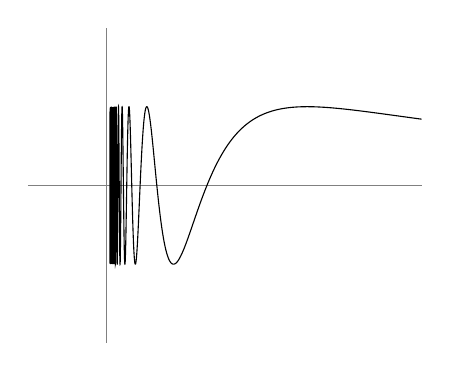
\begin{tikzpicture}
        \draw [help lines] (-1,0) -- (4,0);
        \draw [help lines] (0,-2) -- (0,2);
        \draw [samples=10000,domain=0.04:4] plot ({\x},{sin(deg(4/(\x)))});
      \end{tikzpicture}
      \[\bar{S}=S\cup\set{(1,\sin(1))}\cup\setb{(0,y)}{y\in[-1,1]}\]

    \item Topologists Comb
      \[C=\setb{(x,0)}{x\in[0,1]}\cap\bigcup_{n=1}^{\infty}\setb{\left(\frac{1}{n},1)\right)}{y\in[0,1]}\]

      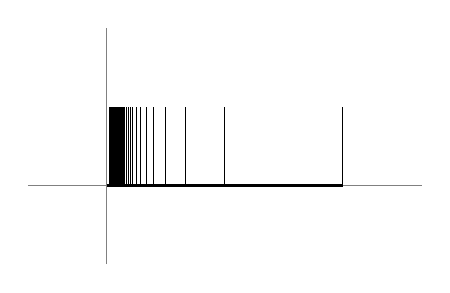
\begin{tikzpicture}
        \draw [help lines] (-1,0) -- (4,0);
        \draw [help lines] (0,-1) -- (0,2);
        \draw [very thick] (0,0) -- (3,0);
        \foreach \n in {1,...,100}{
          \draw ({3/(\n)},0) -- ({3/(\n)},1);
        }
      \end{tikzpicture}
      \[\bar{C}=C\cup\setb{(0,y)}{y\in[0,1]}\]
  \end{enumerate}
\end{example}

\begin{example}
  In \((\R,\T_{\text{std}})\), the Cantor set \(\C\) is a non-empty subset of \([0,1]\) such that:
  \begin{enumerate}
  \item \(\C\) is closed.
  \item \(\C\) contains no non-empty open intervals.
  \item \(\C\) contains no isolated points.
  \end{enumerate}
\end{example}

\end{document}
